\documentclass[xcolor=dvipsnames,10pt,aspectratio=169]{beamer}
%\documentclass[xcolor=dvipsnames,10pt]{beamer}
\usepackage{etex}
\usepackage{pgf,pgfarrows,pgfnodes,pgfautomata,pgfheaps,pgfshade}
\usepackage[absolute,overlay]{textpos} 
%\usepackage{algorithm}
\usepackage{amsmath,amssymb}
\usepackage[utf8]{inputenc} 
\usepackage{colortbl}
\usepackage{graphicx} 
\usepackage[english]{babel}
\usepackage{tabularx} 
\usepackage{multirow}
\usepackage{booktabs}
\usepackage{listings}
%\usepackage{multimedia}
\usepackage{animate}
\usepackage{xcolor}
\usepackage{array}
\usepackage{longtable}
\usepackage{makecell}
\usepackage{caption}
\usetheme{Madrid} 
\usepackage{amsmath}
\usepackage{movie15}


\lstset{ %
%	backgroundcolor=\color{white},   % choose the background color; you must add \usepackage{color} or \usepackage{xcolor}
%	basicstyle=\footnotesize,        % the size of the fonts that are used for the code
	basicstyle=\scriptsize,        % the size of the fonts that are used for the code
	breakatwhitespace=false,         % sets if automatic breaks should only happen at whitespace
	breaklines=true,                 % sets automatic line breaking
	captionpos=t,                    % sets the caption-position to bottom
	commentstyle=\color{mygreen},    % comment style
	deletekeywords={...},            % if you want to delete keywords from the given language
	escapeinside={\%*}{*)},          % if you want to add LaTeX within your code
	extendedchars=true,              % lets you use non-ASCII characters; for 8-bits encodings only, does not work with UTF-8
%	frame=single,                    % adds a frame around the code
	keepspaces=true,                 % keeps spaces in text, useful for keeping indentation of code (possibly needs columns=flexible)
	keywordstyle=\color{blue},       % keyword style
%	language=make,                 % the language of the code
	morekeywords={*,...},            % if you want to add more keywords to the set
%	numbers=left,                    % where to put the line-numbers; possible values are (none, left, right)
%	numbersep=5pt,                   % how far the line-numbers are from the code
	numberstyle=\tiny\color{mygray}, % the style that is used for the line-numbers
	rulecolor=\color{black},         % if not set, the frame-color may be changed on line-breaks within not-black text (e.g. comments (green here))
	showspaces=false,                % show spaces everywhere adding particular underscores; it overrides 'showstringspaces'
	showstringspaces=false,          % underline spaces within strings only
	showtabs=false,                  % show tabs within strings adding particular underscores
	stepnumber=2,                    % the step between two line-numbers. If it's 1, each line will be numbered
}

\definecolor{mygreen}{rgb}{0,0.6,0}
\definecolor{mygray}{rgb}{0.5,0.5,0.5}
\definecolor{mymauve}{rgb}{0.58,0,0.82}

\usecolortheme{beaver}
\newcommand{\ul}{\underline}
\setbeamertemplate{footline}{\scriptsize{\vspace*{0.3cm}\hspace*{15cm}\insertframenumber\,/\,\inserttotalframenumber}}
\setbeamertemplate{caption}[numbered]
\setbeamerfont{caption}{size=\fontsize{8}{5}}

\setbeamercolor{block title}{	bg=Sepia , fg = White}
\setbeamercolor{block body}{bg=Brown!15, fg=Sepia }
\setbeamercolor{item projected}{bg=Sepia, fg=White}
\setbeamercolor{number projected}{bg = Black}

%declara as imagens usadas no layout do slide
\pgfdeclareimage[height=0.8cm]{mflab}{figuras/logo_mflab_transparente.png}
\pgfdeclareimage[height=1.0cm]{logoufu}{figuras/logo_ufu.jpg}
\pgfdeclareimage[height=1.0cm]{petro}{figuras/petrobras_2.png}

%posiciona o logotipo do MFLab
\setlength{\TPHorizModule}{1mm}
\setlength{\TPVertModule}{1mm}
\newcommand{\placelogomflab} 
{ 
	\begin{textblock}{13}(150.0,0.0)
		\pgfuseimage{mflab} 
	\end{textblock} 
	
	\begin{textblock}{13}(150.0,70.0)
		\pgfuseimage{petro} 
	\end{textblock} 
}
\setlength{\TPHorizModule}{1mm}
\setlength{\TPVertModule}{1mm}
\newcommand{\placelogo} 
{ 
	\begin{textblock}{13}(150.0,0.0)
		\pgfuseimage{mflab} 
	\end{textblock} 
	
	\begin{textblock}{13}(0.0,80.0)
		\pgfuseimage{petro} 
	\end{textblock} 
}

\title{NEURAL NETWORK ASSISTED CAVITY CONVECTION FLOW}

\author{ Felipe J. O. Ribeiro \\ \and \\ Prof. Dr. Aristeu da Silveira Neto \\ Prof. Dr. Aldemir Aparecido Cavallini Junior}

\date{\tiny{\today}}
\newcolumntype{C}[1]{>{\centering\let\newline\\\arraybackslash\hspace{0pt}}m{#1}}


\begin{document}

\begin{frame}\placelogomflab
	\frametitle 
	{ \vfill
		\centering
		{
		\small{Federal University of Uberlândia}\\
			% \small{Programa de Pós-Graduação em Engenharia Mecânica}\\
		\small{Fluid Mechanics laboratory}\\
		}
	}
	\maketitle
\end{frame}

\section<presentation>*{Index}
	
\begin{frame}
	\frametitle{Index}\placelogomflab 
	{\scriptsize \tableofcontents}
\end{frame}

\AtBeginSection[]
{
 \begin{frame}<beamer>
  \frametitle{Index}\placelogomflab 
  {\scriptsize \tableofcontents[current,currentsection]}
 \end{frame}
}

\AtBeginSubsection[]
{
 \begin{frame}<beamer>
  \frametitle{Index}\placelogomflab 
  {\scriptsize \tableofcontents[current,currentsubsection]}
 \end{frame}
}


\section{Introduction}

\begin{frame}\frametitle{Objectives}
	\centering
	The present text seeks to document the development of this research work with detail. from mathematical and theoretical developments to progress in technical and organizational aspects.
	\vspace{0.5cm}

	\flushleft
	The core topics of this study are:\\
	\quad $\bullet$ Theoretical and mathematical development of two-dimensional cavity flow;\\
	\quad $\bullet$ Development of artificial neural network machine learning in FORTRAN;\\
	\quad $\bullet$ Enhancement of the visualization methods with OpenGL in FORTRAN;\\
	\quad $\bullet$ Development of MPI methodologies.\\
\end{frame}

\begin{frame}\frametitle{Bidimensional convective flow in a cavity}
	\begin{minipage}[h!]{0.39\textwidth}
		$\bullet$ Natural convection is a classic cavity flow phenomenon. it represents many industrial and everyday situations;\\
		$\bullet$ To simulate such a phenomenon a two or three-dimensional domain is necessary. Which brings new challenges compared to the previous poiseuille flow project;\\
		$\bullet$ Despite dealing with fluid mass changes, the flow is considered incompressible, as volumetric changes are negligible;\\

	\end{minipage}
	\begin{minipage}[h!]{0.6\textwidth}
		\begin{figure}[h!]
			\centering
			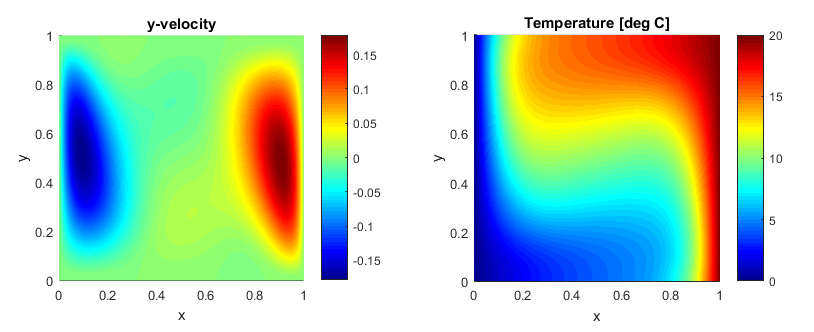
\includegraphics[trim = {0cm 0cm 0cm 0cm}, clip , angle=0, scale=0.45]{./my_images/NaturalConvectionFromNet.png}
			\caption{cavity convection example.}
		\end{figure}
	\end{minipage}
\end{frame}

\begin{frame}\frametitle{Artificial neural network}
	\begin{minipage}[h!]{0.39\textwidth}
		$\bullet$ They seek to mimetize the biology of brains to emulate it's learning capabilities.\\
		$\bullet$ Its based on the neuron entities and it is defined by the structure of neurons and the weights of each connection.\\
		$\bullet$ Training the network, or, the learning process, as it is called, consistis in determining the weights of each connection based on multiples tests and loss calculation. A gradient descent is used to obtain the weights with which the error is the minimal in a given training set.
	\end{minipage}
	\begin{minipage}[h!]{0.6\textwidth}
		\begin{figure}[h!]
			\centering
			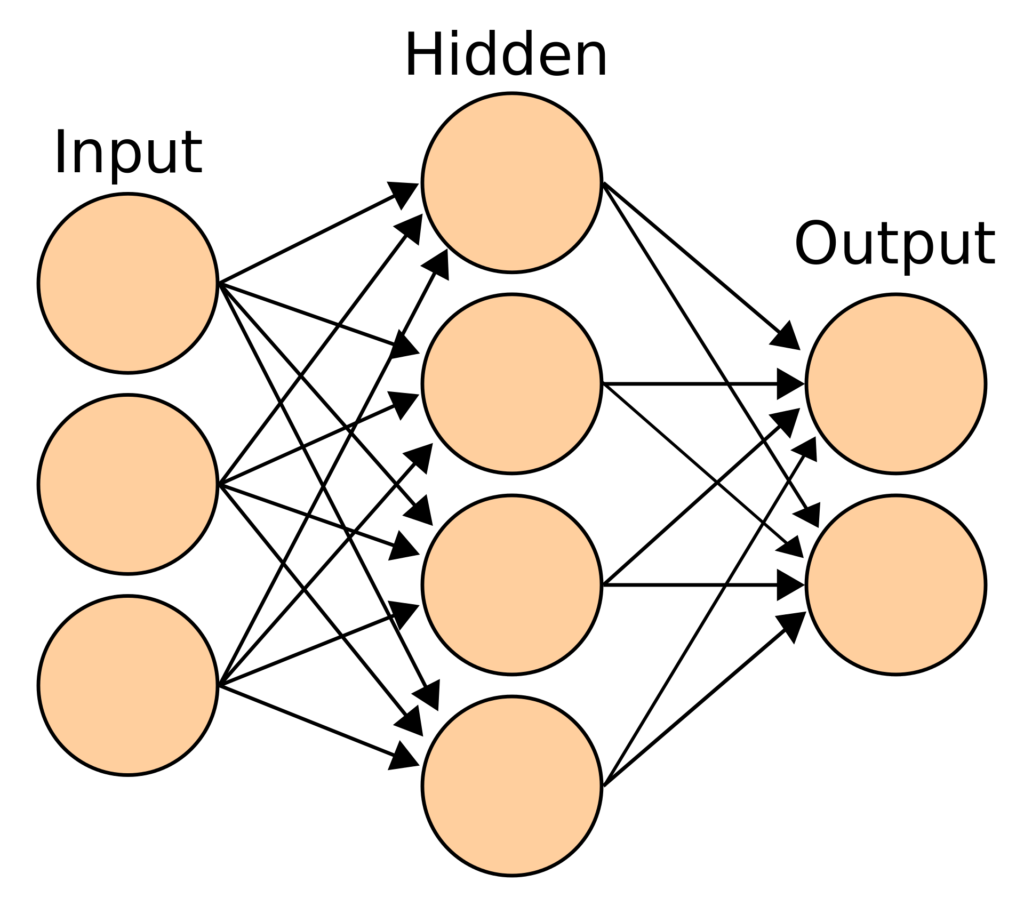
\includegraphics[trim = {0cm 0cm 0cm 0cm}, clip , angle=0, scale=0.18]{./my_images/neural_figure.png}
			\caption{Simple neural network.}
		\end{figure}
	\end{minipage}
\end{frame}

\begin{frame}\frametitle{ANN applyied to cavity flows}
	\begin{minipage}[h!]{0.39\textwidth}
		$\bullet$ Neural netwoks can be described as neural operators that learn mappings between finite-dimensional euclidean spaces.\\
		$\bullet$ The catch is that they are discretization dependent, which drastically affects the applicability of the method.\\
		$\bullet$ As seen in "Fourier Neural Operator For Parametric Partial Differential Equations"... The problem can be solved by training the neural network in Fourier Space.\\
		$\bullet$ Such approach enables the network to be used in a variety of mash sizes and geometries.
	\end{minipage}
	\begin{minipage}[h!]{0.6\textwidth}
		\begin{figure}[h!]
			\centering
			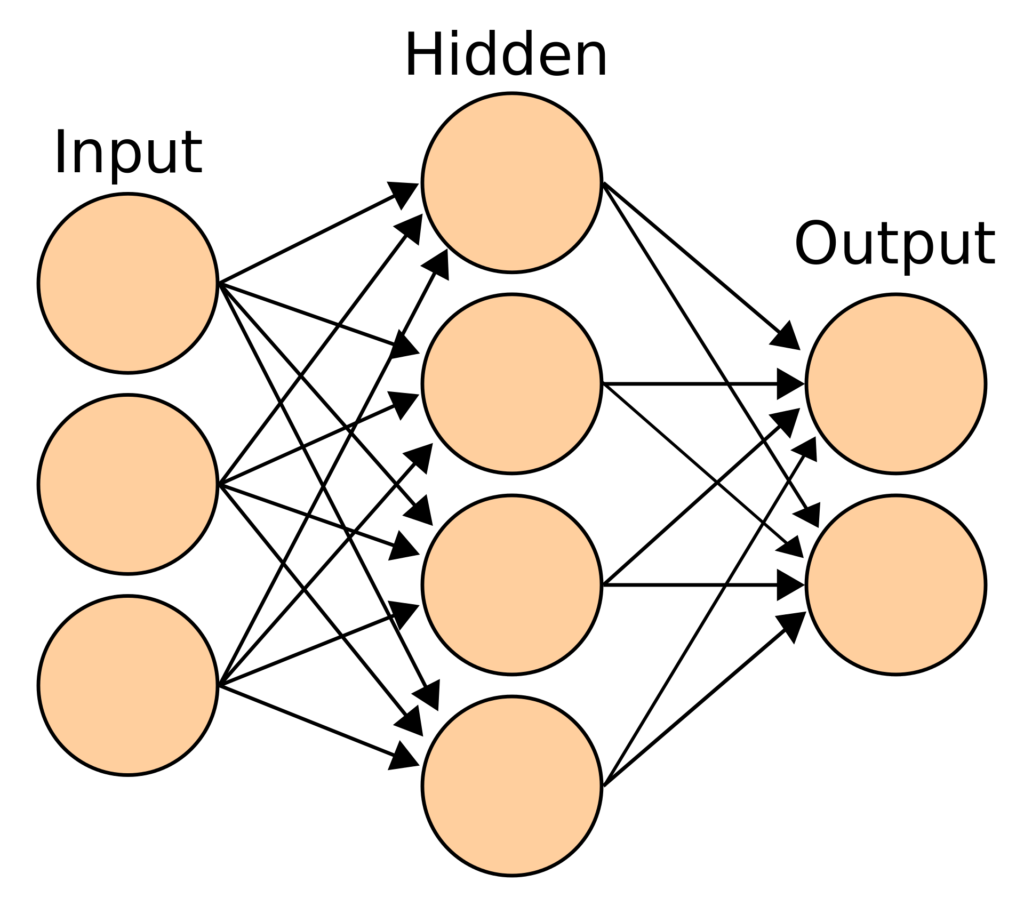
\includegraphics[trim = {0cm 0cm 0cm 0cm}, clip , angle=0, scale=0.18]{./my_images/neural_figure.png}
			\caption{Simple neural network.}
		\end{figure}
	\end{minipage}
\end{frame}

\section{Embasamento Teórico}

\section{Agradecimentos}
	\begin{frame}
		\placelogomflab 
		\frametitle{Agradecimentos}
		\begin{figure}
		\begin{center}
		\begin{tabular}{c c}
			{
\includegraphics[trim=0.0cm 0.0cm 0.0cm 0.0cm,clip=true,height=0.2\textheight]{figuras/petrobras.png}}&{
\includegraphics[trim=0.0cm 0.0cm 0.0cm 0.0cm,clip=true,height=0.2\textheight]{figuras/logo_mflab.png}}\\
			{
\includegraphics[trim=0.0cm 0.0cm 0.0cm 0.0cm,clip=true,height=0.2\textheight]{figuras/cnpq.png}}&{
\includegraphics[trim=0.0cm 0.0cm 0.0cm 0.0cm,clip=true,height=0.2\textheight]{figuras/CAPES.png}}\\
			{
\includegraphics[trim=0.0cm 0.0cm 0.0cm 0.0cm,clip=true,height=0.2\textheight]{figuras/FAPEMIG.jpg}}&{
\includegraphics[trim=0.0cm 0.0cm 0.0cm 0.0cm,clip=true,height=0.2\textheight]{figuras/UFU_black.jpg}}\\
		\end{tabular}
		\end{center}
		\end{figure}
	\end{frame}

	\begin{frame}
		\placelogomflab 
		\frametitle{Agradecimentos}
		\fontsize{44pt}{7.2}\selectfont
		\begin{center}
			Obrigado.
		\end{center}
	\end{frame}
\end{document}
